\subsection{Anomalous Magnetic Moment of the Muon}
We start with the anomalous magnetic moment of the muon since its parameter set only consists of 
\begin{align}
 \left(m, M_l, g_2^l\right).
\end{align}
In general, every charged particle
may have a spin $\boldsymbol{s}$ with an associated magnetic moment \cite{anomMom}
\begin{align}
 \boldsymbol{\mu} = g \frac{e}{2m}\boldsymbol{s}.
\end{align}
The factor $g$ is called the gyromagnetic factor and is equal for all elementary particles of a kind. For fermions it is $g=2$. By saying, the magnetic 
moment is anomalous, one states a deviation from this value which is expressed as $a= (g-2)/2$. There are many contributions to this already within the SM
from QED or hadronic vacuum polarisation which cause most of the uncertainties (1606.06861) but all of them are quantum loop effects. Even when all of them are taken into account, there is still a discrepancy
between theory and experiment 
\begin{align}
 \Delta a_\mu = a_\mu^\text{ex} - a_\mu^\text{SM} = 287(80)\cdot 10^{-11}.
\end{align}
Contributions to $a$ can be evaluated in the following way. An ingoing muon with momentum $p_1$ radiates a photon $A_\mu (q)$, leaving the muon in the final 
state with $p_2$. To first order in the external field, the scattering amplitude is 
\begin{align}
 M = -\ti e \langle \mu_2|J^\mu(x=0)|\mu_1\rangle A_\mu(q),
\end{align}
with the electic current $J^\mu(x)$. The most general parametrisation one can write thanks to Ward identity and parity conservation in QED is for on-shell
($p_i^2 = m_i^2$) external muons
\begin{align}
 \langle \mu_2|J^\mu(0)|\mu_1\rangle = \bar u_2 \left[F_D(q^2)\gamma^\mu + F_P(q^2)\frac{\ti \sigma^{\mu\nu}q_\nu}{2m}\right] u_1.
\end{align}
In the non-relativistic limit, the relation between the magnetic moment and these form factors $F_D$ and $F_P$ can be derived to be
\begin{align}
 \mu = \frac{e}{2m}\left(F_D(0) + F_P(0)\right)
\end{align}
\noindent
with $F_D(0)=1$ but $F_P(0)\neq0$. \cite{Lavoura} provides handy formulae for general one loop electroweak decays as $f_1 \rightarrow f_2 \gamma$. Therein
is $F_P(0) =m_\mu\left( \sigma_L P_L + \sigma_R P_R\right)$ with the $\sigma$s being sums of loop functions. The key process is depicted in figure \ref{pic_g-2}.
\begin{figure}[t]
 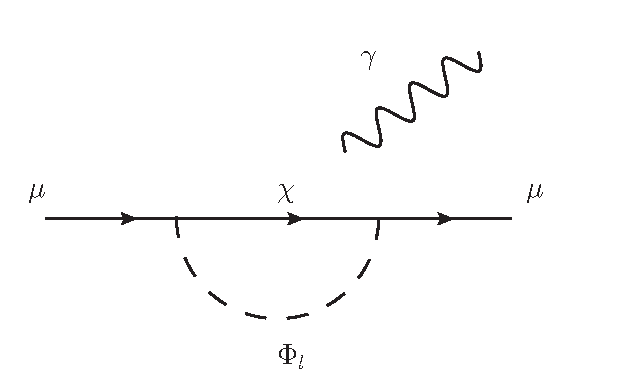
\includegraphics[width=0.6\textwidth]{../pics/g-2.eps}
 \caption{One-loop contribution to $a_\mu$. Depending on the representations, there are multiple possibilites to attach the photon.}
 \label{pic_g-2}
\end{figure}
Since we have a Yukawa interaction coupling to left handed particles, there are only terms left with $\lambda=|g_2^l|^2$, so that we eventually have
\begin{align}
 \Delta a_\mu^\text{NP} = \frac{|{g_2^l}|^2}{16\pi^2}\frac{m_\mu^2}{M_l^2}\left(Q^i_F \frac{1}{x_l}I(x_l^{-1}) + Q^i_B  I(x_l)\right)
\end{align}
with (1503.01500)
\begin{align}
 I(x) = \frac{1}{12(x-1)^4}\left(2+3x-6x^2+x^3+6x\log(x) \right) \stackrel{x\rightarrow1}{=} \frac{1}{24}.
\end{align}
The sum over $i$ is understood so that $Q_\mu = Q_F-Q_B$ is ensured.

there is an i in the electric current and an i in lavoura -> -1